\documentclass[]{article}
\usepackage[utf8]{inputenc}
\usepackage[english]{babel}


\usepackage{geometry}
\geometry{margin=1.3in}


\usepackage{siunitx}
\usepackage{graphicx}
\usepackage{amsmath}
\usepackage{algorithmicx}
\usepackage{multicol}
\usepackage{authblk}

%opening
%\title{Cortical gating is spatially diverse phenomenon for proprioceptive stimulation children and adolescents}
% tai
\title{Distinct gating patterns to different cortical areas for proprioceptive stimulation children and adolescents}
\author[1]{Jaakko Vallinoja}
\author[1]{Timo Nurmi}
\author[1]{Julia Jaatela}
\author[1,2,3]{Harri Piitulainen}
\affil[1]{Department of Neuroscience and Biomedical Engineering, Aalto University School of Science, P.O. BOX 12200, 00076 AALTO, Espoo, Finland}
\affil[2]{Faculty of Sport and Health Sciences, University of Jyväskylä, P.O. BOX 35, FI-40014, University of Jyväskylä, Finland}
\affil[3]{Aalto NeuroImaging, MEG Core, Aalto University School of Science, P.O. BOX 12200, 00076 AALTO, Espoo, Finland}

\date{}
\setcounter{Maxaffil}{0}
\renewcommand\Affilfont{\small}

\begin{document}
\maketitle

\begin{abstract}
Here be dragons.
\end{abstract}


\section*{Introduction}


Sensory gating is a robust well known phenomenon where multiple successive sensory stimuli results in reduction of the respective response amplitudes at the cortex. This is thought to be important to prevent excessive afference and overloading of sensory processing resources in the brain. Sensory gating of auditory responses has been observed to be affected schizophrenia (adler et al????) which has been the main focus of gating studies. Gating in a affected brain is impaired which reduces the suppression of the successive responses. This indicates issues with brain network responsible for processing the response.

%Smeds paperi vastevoimakkuuksista wrt ISI

Double stimulus paradigm where two similar stimuli are presented in quick succession has been used as a systematic tool to study gating in a controlled quantifiable manner. Typically these studies are performed using brief clicks or beeps for auditory or median nerve electric stimulus for somatosensory condition respectively. There are surprisingly few studies about somatosensory gating and even fewer that use a more naturalistic methods than median nerve electrical stimulation. It has been reported that gating in primary somatosensory cortex is not similarly affected by schizophrenia as auditory but that the gating in secondary somatosensory cortex is (edgar et al, thoma et al). 

While gating has been extensively studied with respect to different neural conditions the mechanism is not well known. It is assumed that the gating effect arises from an inhibitory activity initiated by some higher level process. Frontal and thalamic networks have been proposed ??? but there is little evidence for either of them.

Proprioception is the sense of relative position of the body parts. The proprioceptive sensors or proprioceptors are located in muscles (muscle spindles) and tendons (Golgi tendon organ). This information is integrated with the vestibular system to create the overall perception of position and movement of the body. Passive movement stimuli has been used to study proprioception. The goal of the stimulus is to create a sensation of movement and change of position with as little pure tactile stimulation as possible. 

% proprioseptiikkalähde gandevia proske 2012


Proprioceptive stimulation and the respective thalamo-cortical input is known to strongly activate the primary somatosensory (S1) and secondary somatosensory (S2) cortices but is known to activate directly also the primary motor (M1) cortex. When recorded with MEG, the most prominent cortical response for proprioceptive stimulation is seen on the primary sensorimotor (SM1) cortex. Beyond these primary regions, the proprioceptive input is processed within a larger cortical network, including premotor posterior parietal cortices ????. Parts of superior parietal cortex have also been linked to somatosensory shape recognition which involves proprioception. 

%(Piitulainen 2013 ja 2015: https://www.ncbi.nlm.nih.gov/pubmed/23402851 & https://www.ncbi.nlm.nih.gov/pubmed/25770989 )

MEG studies that try to separate neural signals from different cortical regions face several challenges. The inherent point spread of distributed MEG inverse solutions mixes signals spatially in the brain which makes the timeseries in each source point a mixture of true sources. In addition individual neuroanatomical differences between subjects is a challenge when averaging across population especially without some prior knowledge of the differences. In other words, regional specificity is lost if the stimulus response location varies between subjects. Multiple equivalent current dipole fitting approaches would extract spatially separate uncorrelated signals but require prior knowledge of the response such as number of true sources. Furthermore correlated sources that are expected with complex response involving multiple cortical regions would violate the assumptions of equivalent current dipoles. 

In general the goal of MEG inverse solutions is to locate relevant locations and extract source timeseries from the brain. A typical method is to define cortical region(s) of interest based on anatomical criteria and focus on peak response in that area.  Another alternative is to average timeseries over region or extract its first singular vector. All of these approaches have weaknesses. Focusing on the peak location or averaging over the area does not at all address the spreading and overlapping of responses. Simple averaging of a region mixes sources together and the first singular vector method is typically dominated by the globally largest source. Another issue is that the most common anatomy based atlases segment the brain according to most prominent sulci and gyri which does not necessarily reflect functional areas. 

In this work we use an independent component analysis (ICA) approach to determine the relevant source locations and timeseries to proprioceptive double stimuli. ICA has been used in M/EEG analysis in several different ways but typically the goal has been to find independent sources by maximizing temporal sparsity of the components. In this work we instead focus on spatial independence. This method is often used in functional MRI analysis but in MEG it has until now only been used to examine oscillatory activity. Several methods to generalize ICA to group analysis has been proposed. In this work we compute the ica components individually and cluster them over the subjects using spatiotemporal similarity metric.

Our primary aim is to  decompose the proprioceptive gating effect to distinct components and find regions in the brain that could contribute to the gating phenomenon within and beyond the SM1 cortex. 

\section*{Materials and Methods}

\subsection*{Participants}

?? healthy right handed children (ages ??, mean age ??, SD ??) participated in the study. The participants were recruited as a control group to a larger project studying proprioception and cerebral palsy.

\subsection*{Experimental Setup}


\subsection*{Measurements}

MEG measurements were conducted in Aalto University using a 306 channel (204 gradiometers, 102 magnetometers) MEG system (Vectorview, Electa????). The measurement room was magnetically shielded (????) to reduce outside interference. Head position and movement was measured using five head position indicator coils attached to the head. An actuator with a pneumatic muscle (figure ??) was used to elicit passive movement of the index finger. The pneumatic muscle extends roughly 5mm when the pressure inside is quickly dropped from 4 bars to 1 bar. The subjects were to sit as relaxed as possible while watching an uneventful video with slowly moving landscape images. Since the pneumatic machinery caused some small audible noises the subjects wore earplugs and a constant white noise was played to mask the stimulus noises. To reduce tactile stimulation to absolute minimum a light layer of surgical tape was used to cover the fingertip. A cardboard screen was used to cover the fingers so that there would not be visual indication of the movements. The setup is shown in figure \ref{fig:setup}. The measurement was 14 minutes long divided into two 7 minute segments with a small pause between them. The participants did not exit the measurement setup during the pause. Both 7 minute segments contained approximately 55 stimulus pairs for both right and left index finger. 

\begin{figure}
    \centering
    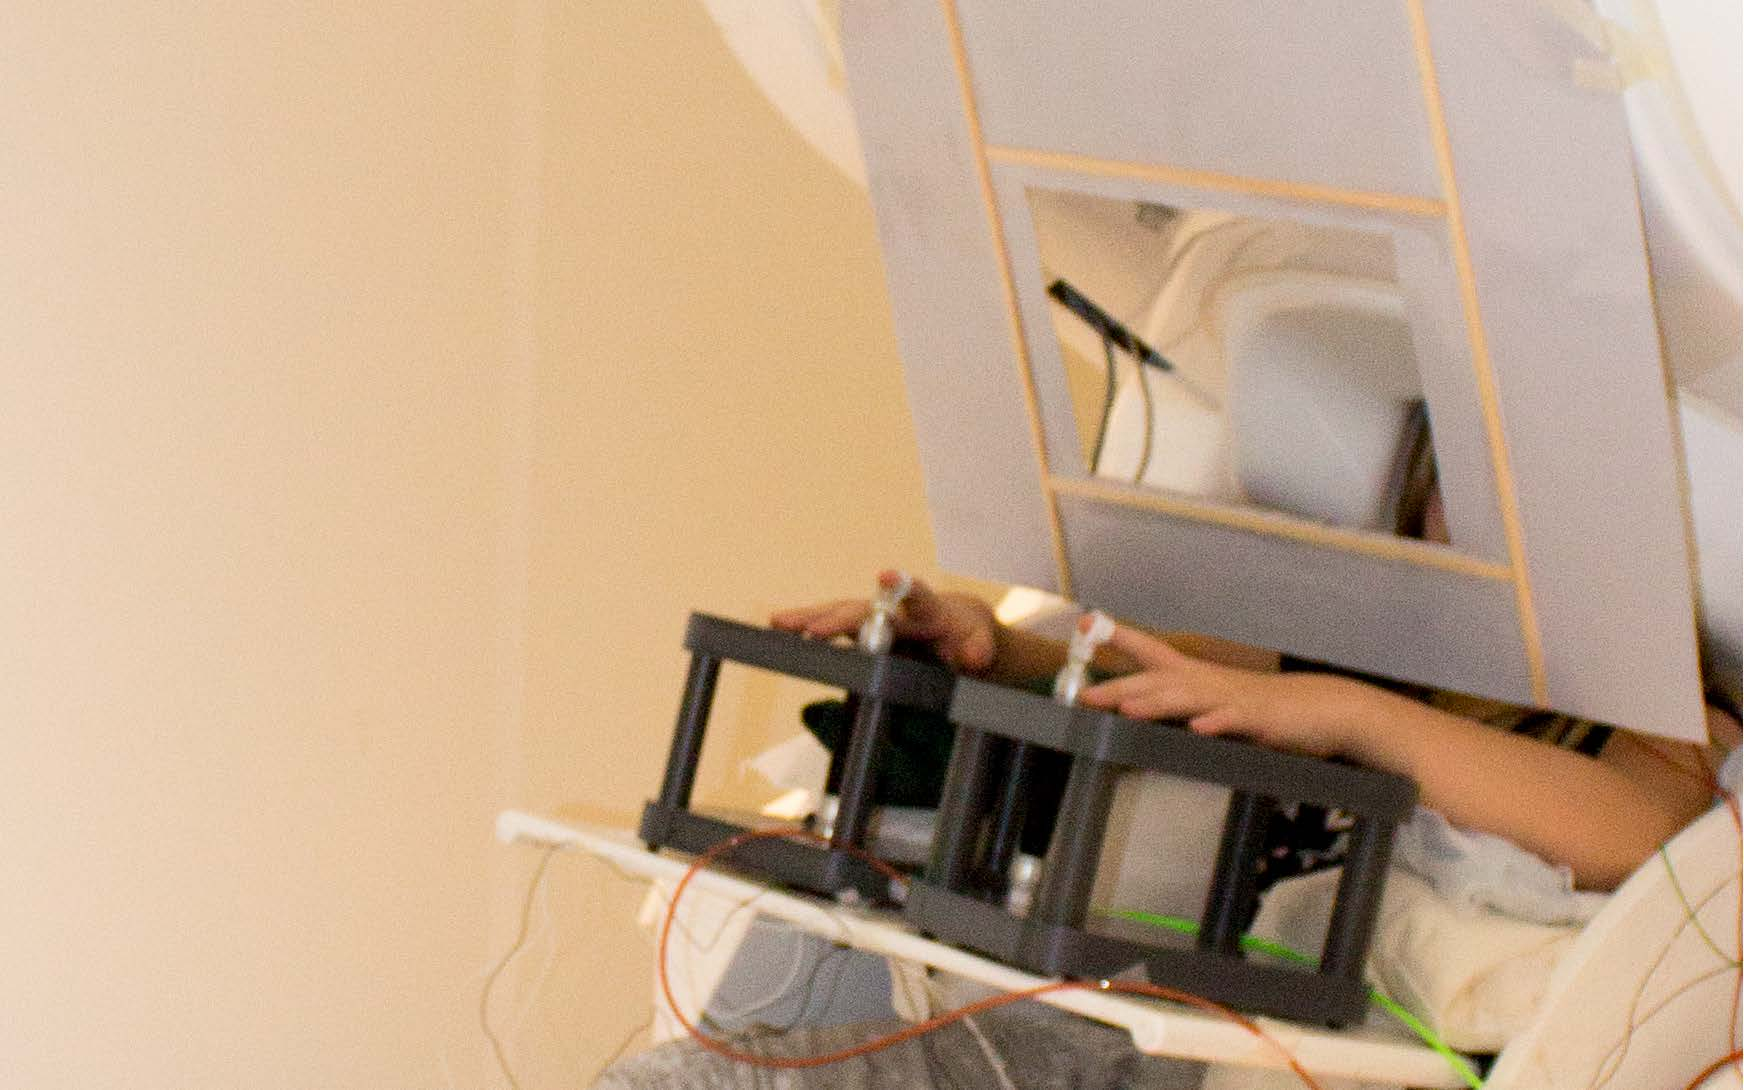
\includegraphics[height=6.5cm]{images/setup.jpg}
    \caption{The measurement setup.}
    \label{fig:setup}
\end{figure}

The stimulus pair consisted of two upward movements of index finger with 500ms interval. There was 4000ms interval with maximum of 250ms jitter between the paired events and the stimulus order between hands was randomized. To quantify the actuator movement we measured it with a laser distance meter and used accelerometers to check that the movement was similar between subjects. No significant variation was detected in the stimulus between sessions. Actuator movement pattern is presented in figure \ref{fig:actuator-movement}. 

\begin{figure}
    \centering
    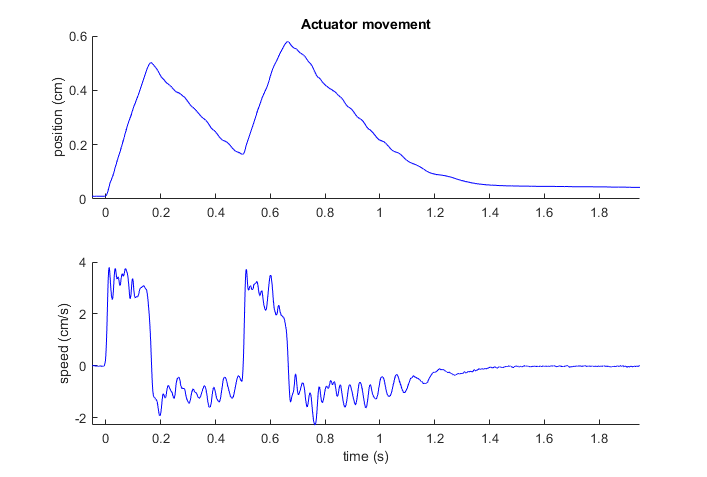
\includegraphics[height=6.5cm]{images/actuator_movement.png}
    \caption{The displacement and speed of the pneumatic actuator measured with a laser distance meter.}
    \label{fig:actuator-movement}
\end{figure}

\subsection*{MEG Preprocessing}

MEG data was first denoised using oversampled temporal projection (OTP, taulu, mne-python). This novel method assumes the data is spatially oversampled and reconstructs each sensor data using the other sensors. This means that sensor related uncorrelated noise and artefacts are effectively removed. After OTP denoising temporal sub space separation (TSSS, Electa Maxfilter) was used to remove interference coming from outside the head. Maxfilter process also corrected the head movement and filtered the HPI coil signals from the data. 

ICA (hyvärinen ????) was used to separate ocular artefacts from the data. 30 components were computed and the artefact components were chosen by correlating with reference electrode measurement. While TSSS had removed most cardiac activity from the signal some residual was found with ICA and those components were also removed. All removed components were checked manually.


\subsection*{Source Location Analysis}

A high resolution structural MRI scans (T1 and T2 mprage etcetc ????) was taken for each participant. MRI data was collected using 3-T Siemens Skyra MR scanner. Freesurfer software (????) was used to construct brain a surface model for each participant. MNE software (????) was used to create a surface based source space with 8196 source vertices with average of less than 5mm distance between them. Each vertex represents a point with three orthogonal dipoles. MNE software was used to create the MEG forward solutions for the source spaces.

The source activity estimation was done using the well know dSPM method (Dale et all???) which is a minimum norm estimate normalized with pre stimulus activity. The MNE-python implementation of the algorithm was used. A minimum norm approach was chosen because we do not want to make any a priori assumptions on the nature of the source distributions. Especially since with passive movement stimulus we can expect highly correlated activity in multiple brain regions. The inverse solution had depth weighting of 0.8 and dipole orientation was loosely weighted for surface normal (with weighting parameter 0.3). The noise covariance was estimated from 0.5 second periods before each double stimulus event. 

%the other option
%The source activity estimation was done using a linearly constrained minimum variance (LCMV) beamformer implemented in the MNE-python tools. A beamformer solution should give fairly well localized and focal solutions for uncorrelated sources. 

MEG data was band pass filtered between 1 and 40 Hz and downsampled to 100Hz sampling. The data was epoched to baseline corrected epochs -0.2 -- 1.2 seconds around the stimuli of interest (right index finger movement). Each subject data was time shifted so that the response onset was at zero. This was done to equalize the differences in neural conduction times between subjects that were at various points of growth in puberty. To standardize the amount of data between the subjects and conditions, a random permutation of 90 epochs were chosen for each subject. Source estimation was done without averaging the epochs because averaging would violate the assumptions of ICA that will be used for data analysis. The entire three dimensional vector solution was estimated. This resulted in $3\times8196 = 24588$ timecourses per subject. 

\subsection*{Independent component analysis}

The properties of TSSS algorithm used in preprosessing cause the true rank of our 306 channel MEG data to be around 70. ICA behaves badly on rank deficient data so it is necessary to reduce the data dimensionality. This is obviously beneficial for computational purposes too. We use truncated singular value decomposition to get 65 timecourses (right singular vectors) and their respective spatial source topographies (left singular vectors) instead of 24588 timecourses in 8196 source points. 65 components were enough to explain more than 98\% of the variance in all subjects. It is an open question if data should be reduced further to remove noise components. However the unaveraged response signal to our proprioceptive stimulus is relatively small compared to noise components so significant data reduction risks losing information. %In fact with several subjects it was difficult to find consistent response shapes or fit reasonable dipoles to evoked responses. 


%TODO find out the standard way for the equations
\begin{equation}
X = \tilde{U} \tilde{\Sigma} \tilde{V}^T +  \tilde{U}_e \tilde{\Sigma}_e \tilde{V}_e^T
\end{equation}
$\tilde{U}$ contains 65 orthogonal spatial topographies and $\tilde{V}$ the corresponding 65 timecourses.


The ICA analysis approach we use roughly follows ideas presented for example in ????. ???? also did similar analysis to find neural sources from evoked responses but using temporal ICA. The singular vectors from SVD represent spatial and temporal low rank subspaces of the data. In this work the ICA is applied to spatial side. Spatial ICA (SICA) is frequently used in fMRI analysis but less in MEG probably because MEG ICA analysis has largely concentrated on sensor space and the number of sensors provides few sample points for ICA. Also the signals in sensor space are very highly spatially overlapping making meaningful separation more difficult. In source space the signals are easier to spatially separate and the model is simpler to justify physically. Furthermore the assumption that the neural sources are spatially separable is more intuitive than the assumption that the components of a complex stimulus response are temporally independent. In recent years there have been several works applying SICA to Hilbert envelopes of oscillatory resting state activity but we don't know of anyone trying application to evoked responses.

%todo think this through. it is i think more like the timeseries being the random vectors that produce different values for each spatial point... maybe. shit this is difficult %TODO TODO think this through not quite correct atm!!!
In general SICA can be understood to look for components that are minimally spatially overlapping. Each source distribution is thought to be a sample from a set of random vectors with unknown mixing matrix and the ICA tries to find a set of distributions that can be used to reproduce the data with minimal overlaps. %Similar idea is used in MOCA (??) using the imaginary part of fourier transformation of the signal.

We use FastICA algorith to estimate 65 independent components. The components are given by
\begin{equation}
S_s = \tilde{U} W  
\end{equation}
where $W$ is the ICA unmixing matrix. The respective average timecourses can then be found by using the mixing matrix $W^{-1}$
\begin{equation}
	S_t = W^{-1} \tilde{\Sigma} \tilde{V}_{ave}
\end{equation}
where $\tilde{V}_{ave}$ is the average evoked response projected to the space defined by $\tilde{U}$.

%TODO check MNI template info
The components are scaled so that the peak spatial magnitude (norm of the three vector directions) of each component is 1. Finally the topographies $S_s$ are transformed to common MNI152 template brain for group comparison purposes. The temporal components $S_t$ and the MNI-transformed spatial components $S_s$ are stored for each subject and used for clustering.


\subsection*{Component clustering}

We assume that the components from different subjects should have spatiotemporal similarities if they represent real brain activity. Thus we should be able to find component clusters that represent the relevant stimulus responses. While dimensionality reduction before ICA might have been problematic we can at this phase reject many components that don't seem to present stimulus related activity. We rank the components of each subject according to post stimulus amplitude normalized with the pre stimulus standard deviation. We then pick 40 best components from each subject and discard the rest.

The spatial similarity measure we use is simply the traditional Pearson correlation of the spatial distributions of the components. Notably we estimate the independent components in three dimensional vector space but compute the similarities from component magnitude in each location. This choice was made because we are more interested in the approximate location than the exact dipole direction on the variable sulci of each brain. The three dimensional vector components are approximately orthogonal and thus have zero spatial similarity within subjects. However the vector magnitudes of the components are not orthogonal so two components that have spatially overlapping locations will have non zero similarity even within subject.

\begin{equation}
	SM_{s \, X,Y} = \rho_{X, Y} 
\end{equation}

For temporal similarity we use the absolute Pearson correlation of the averaged component timecourse. Because there might be individual differences for the exact response timing between the subjects we find the largest correlation with maximum lag of $\SI{10}{\milli\second}$ between signals. 
\begin{equation}
SM_{t \, X,Y} = \max_\tau{\lvert\rho_{X(t), Y(t+\tau)}\rvert}, \quad \tau \in [\SI{-10}{\milli\second}, \SI{10}{\milli\second}]
\end{equation}
Allowing the lag might overestimate the similarity between higher frequency oscillating sources but in this study we are interested in responses that are clearly stimulus related so the high frequency oscillatory components can be discarded.


We are looking for components that are similar both spatially and temporally. To this end we use weighted geometric mean of spatial and temporal similarities to compute the final similarity matrix. Using the geometric mean as compared to arithmetic mean will both equalize the effect of spatial and temporal similarity and increase distance between components that are similar only spatially or temporarily and not both. Similarity matrix is
\begin{equation}
	SM_{st} = \exp \{ \alpha \times \ln(SM_s) + (1 - \alpha) \times \ln(SM_t) \} 
\end{equation}

where $\alpha \in [0,1]$ determines the weighting between spatial and temporal similarity. In this work we used $\alpha = 0.75$ because we wanted rather strictly spatially similar components but any other value could be used to reflect the preference between spatial and temporal similarity. We get the dissimilarity matrix 
\begin{equation}
D = \sqrt{1 - SM_{st}}
\end{equation}

\begin{figure}
    \centering
    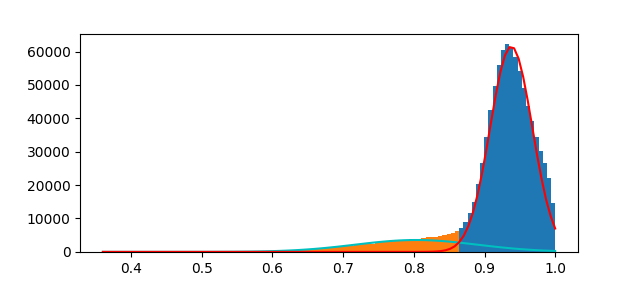
\includegraphics[height=5.5cm]{images/distance_distributions.png}
    \caption{The distribution of inter component distances. The highest mode is thought to represent random similarities and the long left tail includes the interesting correlations. A gaussian mixture model presented by the curves was used to estimate the threshold for clustering.}
    \label{fig:distance-distribution}
\end{figure}

The clustering method used is somewhat similar to the ones described in ?? and ??. It is a semi supervised  agglomerative clustering algorithm that adds components one by one to nearest cluster making sure there is only one component from each subject. The algorithm adds components to their closest cluster provided that the cluster doesn't already have a component from the same subject and the distance to all cluster members is below a threshold. Clusters are combined to their nearest neighboring clusters if they don't have components from the same subjects and the distance between all the cluster members is below the threshold. This is done until all remaining distances are over the threshold. The result is a set of clusters with all intra-cluster distances below the threshold. We pick the clusters that have a component from at least two thirds of the subjects as group representatives. 

The choice of clustering threshold was done by looking at the distribution of inter component distances shown in figure \ref{fig:distance-distribution}. The distribution has a long left tail that can be thought to represent the interesting similarities while the large mode is the random correlations. We fitted a mixture model of two gaussians to the distribution and picked the point where the left distribution becomes more probable as the threshold.


The timecourses and spatial topography for each cluster is averaged to produce the components representing the group. Because of the sign ambiguity the timecourses are flipped to best matching direction. To lessen the effect of small individual variations we use the same $\SI{10}{\milli\second}$ time matching that was used in the similarity computation. 

The criteria for the components of interest to be selected for further examination included 1. the component represents more than two thirds of the subject and 2. the component has clear stimulus related activity (difference between baseline and stimulus). We also put the greatest emphasis on the components in the known sensory-motor areas.

The resulting cluster timecourses are also compared to corresponding anatomical label timecourses in the typical grand average solution.


\section*{Results}
%TODO writing is easier when the pictures are added. now it's more just structure planning

The clustering resulted in 33 (TODO check final) clusters with 18 -- 24 components from individual subjects in each cluster. 

The resulting clusters are most well defined both spatially and temporally in the somatomotor areas of the brain. Figure ?? shows components picked from around the contralateral central sulcus representing the primary sensory and motor areas. Figure ?? shows components around the contralateral posterior lateral sulcus and inferior parietal areas. The respective areas for ipsilateral side are shown in figures ?? and ??. Further interesting components were found in superior parietal and frontal areas shown in figures ?? and ??.

%todo side by side images
%\begin{figure}[h!]
%	\centering
%	\includegraphics[height=10cm]{results1}
%\end{figure}

Figure ?? shows the peak location of grand average evoked activity. ?? show the first PCA timecourses extracted from anatomical areas. 



\section*{Discussion}

It is clear that a signal source separation based approach like the one used can extract features that would otherwise be covered by the primary responses extended by the point spread of the inverse solution. 

Spatial ICA offers the benefit of not assuming the separate sources in the brain being temporarily independent. However the primary concern with this method is the difficulty of interpreting ICA results. The FastICA algorithm acts essentially as a black box and it is very hard to discern what exactly causes it to end up with a particular separation. Furthermore FastICA as a gradient descend based algorithm inherently cannot say if it has found the global optimal solution. There are possible methods to mitigate this (e.g. icasso ????). But no best practice has been established. Spatial ICA with stimulus related MEG data seems to find mostly fairly focal distributions with clear modes which could imply approximately dipolar sources in those locations. Showing this is actually the case is not easy and it is likely that strong sources that are dominant in large areas of the source spaces are at least partly leaked to multiple components. We cannot assume a true separation of original sources can be achieved without additional information. Also the properties of the inverse solution affect the separation significantly. Localization errors affect the activity distribution and consequently the separation of components.

In this study we chose to do group analysis by using individual ICA and clustering. Another common approach to group ICA problem is to concatenate the data from all the subjects and do dimensionality reduction and ICA to that group data matrix. This approach is simpler and offers the additional benefit of making it trivial to project back to check how each subject contributes to each component. However the differences in the exact locations of the hand representative area would make the analysis difficult in our problem. It is likely that the anatomical and physiological differences would affect the component separation. The clustering approach allows more variability in the functional anatomy if the brain as the components don't need to be exactly the same in each subject. 

The main problem with the clustering approach, at least in this study, is that the clustering result is sensitive to the methods and parameters used. We used data driven approach to choose the clustering threshold but by adjusting it the clusters can vary significantly. Some of the clusters are spatially and temporally fairly similar and with slightly different parameters we get different divisions of components between them. Partly this is caused by the strict limitation of just one component per subject in a cluster. Two clusters that perhaps should be combined may not be because they both already contain a component from the same subject. This makes it also harder to interpret the results in terms of gating ratios. We can say that different cortical processes are differently affected by the gating effect but different clustering results would produce different average shapes for components. 

However even with all the methodological difficulties the spatial ICA seems to find many components that are very hard to find from a simple group averaged response.

Many methodological studies to MEG processing are done using a very clear strong stimulus. A neural electric stimulus produces a clear consistent response as does an auditory beep stimulus. Our finger movement evoked a weak response with seemingly variable average shape. It is possible also that the study setting had small variations between subjects that affected how much tactile activation was involved.


\end{document}
